%%%% AAAI-27 anonymous submission -- SHORE-RL
%%%% Style files: aaai2027.sty / aaai2027.bst (official AAAI-27 author kit, v2027/05/04)
%%%% Build:  pdflatex main ; bibtex main ; pdflatex main ; pdflatex main
%%%% NOTE: this is a WORKING DRAFT. Items marked \todo{...} need experiments/checks
%%%%       before this is submission-ready. Main empirical claim = sustained
%%%%       final-window performance on long-horizon tasks.

\documentclass[letterpaper]{article} % DO NOT CHANGE THIS
\usepackage[submission]{aaai2027}  % anonymous submission version
% aaai2027.sty loads the required newtxtext, helvet, and courier fonts.
\usepackage[hyphens]{url}  % DO NOT CHANGE THIS
\usepackage{graphicx} % DO NOT CHANGE THIS
\urlstyle{rm} % DO NOT CHANGE THIS
\def\UrlFont{\rm}  % DO NOT CHANGE THIS
\usepackage{natbib}  % DO NOT CHANGE THIS AND DO NOT ADD ANY OPTIONS TO IT
\usepackage{caption} % DO NOT CHANGE THIS AND DO NOT ADD ANY OPTIONS TO IT
\frenchspacing  % DO NOT CHANGE THIS
\setlength{\pdfpagewidth}{8.5in} % DO NOT CHANGE THIS
\setlength{\pdfpageheight}{11in} % DO NOT CHANGE THIS

\usepackage{amsmath}
\usepackage{amssymb}
\usepackage{booktabs}
\usepackage{multirow}

\pdfinfo{
/TemplateVersion (2027.1)
}

\setcounter{secnumdepth}{2}

% ---- float placement: let more floats land near their text ----
\setcounter{topnumber}{3}
\setcounter{totalnumber}{4}
\renewcommand{\topfraction}{0.9}
\renewcommand{\textfraction}{0.05}
\renewcommand{\floatpagefraction}{0.7}

% ---- draft-only helper (remove before submission) ----
\newcommand{\todo}[1]{\textbf{[TODO: #1]}}
\newcounter{algorithm}

\title{SHORE-RL: Shortening the Horizon for Long-Horizon Residual\\
Reinforcement Learning}

\author{Anonymous Submission}
\affiliations{}

\begin{document}

\maketitle

\begin{abstract}
Behavior-cloned manipulation policies, including modern vision-language-action (VLA)
models, are strong but bounded by the quality of the demonstrations they imitate. Freezing such a cloned
base policy and learning a small additive residual with off-policy RL is an effective way to
improve beyond this ceiling. On long-horizon manipulation, however, the
evaluated RL-finetuning methods fail to sustain improvement and finish below
the frozen base policy. \textbf{SHORE-RL} addresses this late-training collapse
by reducing the long horizon to a sequence of short ones, so that each residual
correction is conditioned on a nearby, self-derived target rather than only on
a long, sparsely rewarded trajectory. SHORE-RL is a base-policy-agnostic
plug-in: a navigator extracts latent waypoints (\emph{where to go}) from a
goal-conditioned value learned on frozen base-policy features, without
object-pose or goal-distance inputs, while a separate critic-reward path
provides dense progress feedback (\emph{how well the policy is doing}). In
simulation, SHORE-RL achieves high and sustained success rates on four
long-horizon DexMimicGen tasks, while action-space residual, noise-space,
imitation-bootstrapped, and full-policy RL baselines collapse below their
frozen base policies. The same plug-in also improves a frozen $\pi_0$ policy
on LIBERO. On a real robot, residual training in world-model imagination
improves success over the frozen base policy on three long-horizon tasks.
\end{abstract}

% =====================================================================
\section{Introduction}
% =====================================================================
Behavior-cloned (BC) manipulation policies provide a strong control prior, but they
inherit the errors and coverage limits of their demonstrations~\cite{ross2011dagger,mandlekar2021matters}. Residual
reinforcement learning (RL) offers a parameter-efficient route beyond this ceiling:
it freezes the pretrained policy and learns only a bounded additive action
correction~\cite{johannink2019residual}. Recent frozen-policy adaptation methods show
that restricting the trainable component can make online finetuning substantially
more sample efficient~\cite{ball2023efficient,resfit2025residual}. This restriction,
however, acts on the \emph{adaptation space}, not its temporal span: ResFit
still optimizes every local correction from the task-level return over the remaining
episode.

We study late-training collapse in long-horizon residual finetuning. Across the
evaluated methods, some policies improve transiently whereas others degrade
earlier, but their long-horizon performance eventually falls below the same
frozen base reference. In a controlled horizon comparison, ResFit remains
stable on the shorter-horizon task but collapses on long-horizon, sparsely
rewarded manipulation. This pattern identifies extended temporal composition
as the central empirical factor in our setting. Sparse delayed
feedback~\cite{arjona2019rudder} also provides a mechanism-level explanation:
each correction receives weak local evidence of whether it helps, while critic
error and residual drift can accumulate over the remaining trajectory. We use
this analysis to motivate the design, not to claim that any one mechanism is
the independently established cause of collapse.

Our central question is whether residual finetuning can remain stable on
long-horizon, sparse-reward tasks by shortening the effective objective horizon
faced by each correction. We separate two roles. On the actor path, a nearby
latent waypoint conditions the residual policy and localizes its target. On the
critic path, an independent progress signal supplies dense shaped rewards; it
neither consumes the waypoint nor evaluates waypoint progress. Learning curves
identify late-training collapse, and final-window success rate summarizes
whether an improvement is sustained.

We introduce \textbf{SHORE-RL}, a horizon-shortening framework for frozen-policy
residual adaptation. A navigator learned from demonstrations proposes latent waypoints
from frozen base-policy features, without simulator-only object poses, goal
coordinates, or geometric distance-to-goal signals. These waypoints condition the
residual actor and critic but remain separate from reward construction. A
separate path supplies dense rewards only to the TD3 critic:
the main simulation study uses a hand-designed per-stage bonus, and a
self-derived alternative uses differences of a learned single-state potential.
The goal-conditioned waypoint value and learned potential remain functionally
independent. We finally study real-robot learning through a learned dynamics
model as an extension of the same residual objective.

\begin{figure*}[t]
\centering
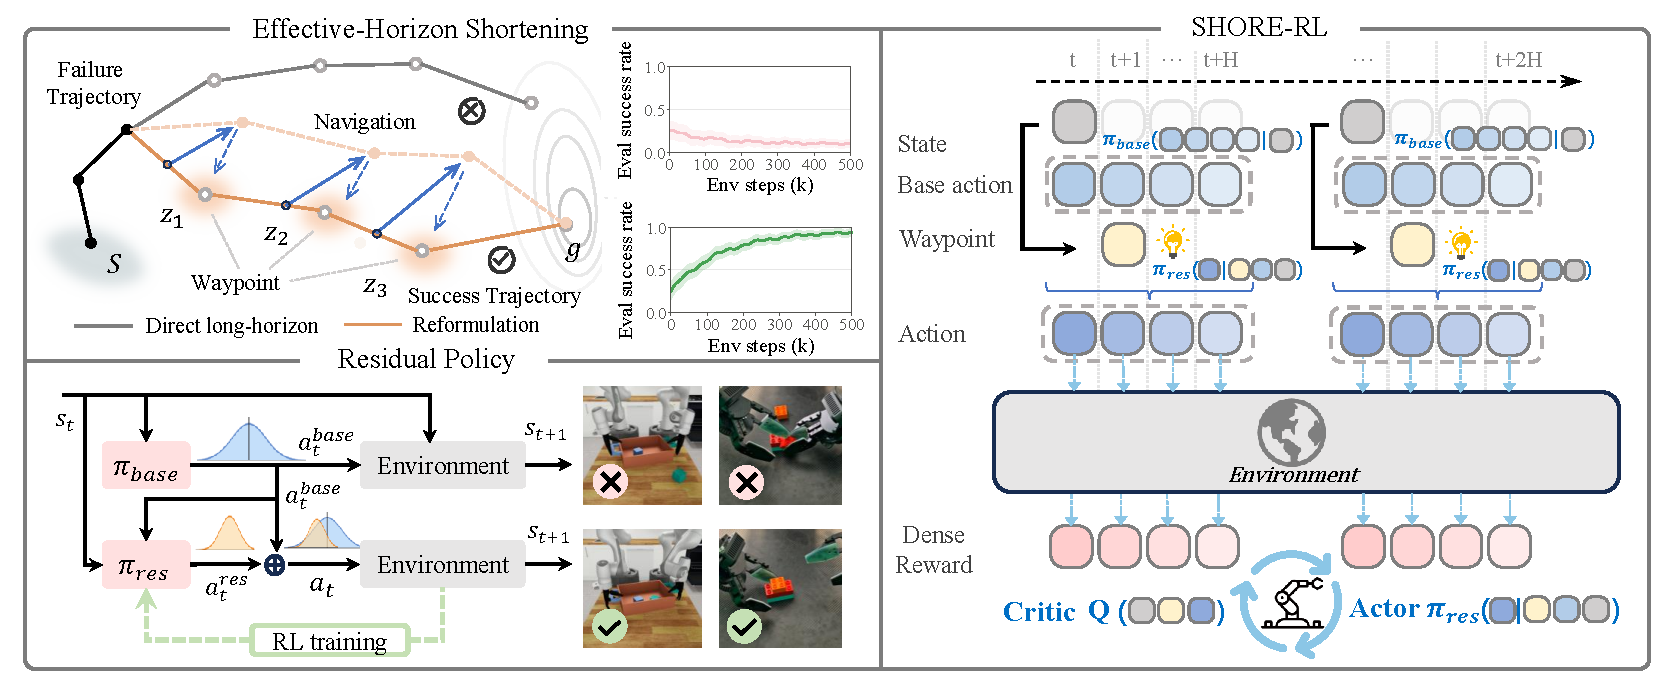
\includegraphics[width=\textwidth]{figure/framework.pdf}
\caption{\textbf{Overview of SHORE-RL.}
\emph{Upper left:} Direct long-horizon navigation provides weak local feedback
and can lead to a failure trajectory, whereas latent waypoints shorten the
effective horizon by decomposing the task into local navigation segments.
\emph{Lower left:} In the overall residual-RL framework, the frozen base policy
and the trainable residual policy jointly produce the executed action, and
environment transitions are used for residual-policy training. \emph{Right:}
SHORE-RL instantiates this framework over successive action chunks. A navigator
predicts a latent waypoint that conditions the residual actor, while an
independent dense progress reward trains the TD3 critic without consuming or
evaluating the waypoint.}
\label{fig:framework}
\end{figure*}

\paragraph{Contributions.}
\begin{enumerate}
\item \textbf{A long-horizon failure pattern and mechanism analysis.} We show
empirically that existing RL-finetuning methods fall below their frozen bases
on long-horizon tasks while ResFit remains stable on a shorter-horizon control.
We connect this pattern to sparse delayed credit and the accumulation of critic
error and residual drift, and quantify sustained performance with final-window
success rate.
\item \textbf{Waypoint-conditioned residual RL.} To our knowledge, SHORE-RL is
the first RL-finetuning method to use latent waypoints to shorten the objective
horizon of a frozen-base residual. It is a base-policy-agnostic plug-in that
requires neither simulator-only object poses, goal coordinates, nor geometric
distance-to-goal inputs.
\item \textbf{Evidence across tasks and base policies.} We evaluate sustained
performance against action-space, noise-space, imitation-bootstrapped, and
full-policy baselines on long-horizon manipulation, test the plug-in with ACT
and $\pi_0$, compare a stage bonus with a stage-detector-free learned
potential, and extend the residual objective to real-robot imagination.
\end{enumerate}

% =====================================================================
\section{Related Work}
\label{sec:related}
% =====================================================================
\paragraph{RL Finetuning of Imitation Policies.}
Behavior cloning provides a strong initialization for robot control but remains limited
by demonstration quality and coverage~\cite{ross2011dagger,mandlekar2021matters}. Online RL can improve this initialization, and
prior-data methods improve sample efficiency by mixing demonstrations with newly
collected transitions~\cite{ball2023efficient,nakamoto2023calql,zhang2023pex,li2023explore}. IBRL retains the imitation policy as an
action proposal and uses learned values to choose between imitation and RL
actions~\cite{hu2023imitation}. These methods primarily address initialization, data
reuse, or how strongly the learned policy remains anchored to imitation. Our focus is
sustained final-window performance when temporal composition is extended.

\paragraph{Residual and Latent-Space Policy Adaptation.}
Residual RL freezes a controller and learns an additive action
correction~\cite{johannink2019residual,yuan2025policydecorator}. ResFit applies this parameterization to
behavior-cloned manipulation policies and combines it with sample-efficient off-policy
learning from prior data~\cite{resfit2025residual,ball2023efficient}. DSRL instead
optimizes the initial noise of a frozen diffusion or flow policy, moving adaptation
into a latent sampling space~\cite{wagenmaker2025dsrl}. These approaches differ in the
\emph{space} in which adaptation occurs and in how it is constrained around the base~\cite{ren2025dppo}.
They do not provide each residual correction with a temporally local objective.

\paragraph{Temporal Abstraction and Progress Shaping.}
Temporal abstraction decomposes a long task into intermediate
goals~\cite{nachum2018hiro,fang2022ptp,shi2023skimo,zheng2024prise}. HIQL, for
example, learns a high-level latent subgoal together with a learned low-level
policy that reaches it~\cite{park2023hiql}. Existing RL-finetuning methods for
frozen imitation policies instead adapt actions, latent noise, or action
selection without using waypoints to shorten the residual objective horizon.
SHORE-RL fills this gap by conditioning only the frozen-base residual on a
value-ranked future feature. Progress shaping is complementary:
transition-level feedback may come from a stage bonus or from potential
differences~\cite{ng1999policy,devlin2012dynamic}.

\paragraph{World-Model Robot Learning as an Extension.}
Learned dynamics models provide policy-learning experience when direct robot
interaction is expensive~\cite{hafner2020dreamer,janner2019mbpo,hansen2024tdmpc2,mazzaglia2023choreographer}.
RISE uses an action-conditioned video model for robot policy
improvement~\cite{yang2026rise,escontrela2023viper}. We similarly use learned
dynamics as a training environment, while retaining the same frozen-base
residual objective.

% =====================================================================
\section{Preliminaries}
% =====================================================================
\paragraph{Problem setting.}
We consider an episodic partially observable control problem with observation
history $o_{\leq t}$, action $a_t$, task reward $r_t$, discount
$\gamma\in[0,1)$, and horizon $T$. The objective is the expected discounted
task return. A frozen behavior-cloned policy $\pi_b$ proposes an action or
flattened action chunk $a_t^b$. Residual
adaptation~\cite{resfit2025residual} keeps this base policy frozen and learns
a bounded correction, instantiated by SHORE-RL in Section~\ref{sec:hier}.

\paragraph{Goal-conditioned learning.}
HIQL~\cite{park2023hiql} learns an action-free goal-conditioned value by
expectile regression,
\begin{equation}
\mathcal L_V
=
\mathbb E\!\left[
\ell_2^\tau\!\left(
 r_g+\gamma m_g\bar V(s_{t+1},g)-V(s_t,g)
\right)\right],
\label{eq:hiql-value-background}
\end{equation}
where $g$ is a sampled goal, $r_g$ is the goal-reaching reward, $m_g$ is its
continuation mask, $\ell_2^\tau$ is the expectile loss, and $\bar V$ is a
slow target. A high-level policy can then be extracted by advantage-weighted
regression over future states; Section~\ref{sec:value} instantiates this
construction only for the SHORE-RL navigator.

\paragraph{Potential-based reward shaping.}
For a fixed state potential $\Phi$, potential-based reward
shaping~\cite{ng1999policy} uses
\begin{equation}
 r_t^\Phi=r_t+\gamma\Phi(s_{t+1})-\Phi(s_t),
\label{eq:pbs-background}
\end{equation}
where $s_t$ is a generic state. With a zero terminal potential, this
transformation preserves the standard discounted objective; the frozen
SHORE-RL potential is defined in Section~\ref{sec:pot}.

% =====================================================================
\section{Method: SHORE-RL}
% =====================================================================
Figure~\ref{fig:framework} summarizes SHORE-RL: a frozen base policy proposes
the nominal action, a base-feature navigator supplies a latent waypoint to
the residual actor and critic, and a separate reward constructor supplies
dense critic feedback without consuming or evaluating the waypoint.
Algorithm~\ref{alg:shore-sim-libero} composes these modules into the residual
rollout and off-policy optimization loop.

\subsection{Horizon-Shortening Residual Policy}
\label{sec:hier}
At each decision, the base policy proposes $a_t^b$, the navigator produces
$z_t$, and the residual actor samples
$\delta_t\sim\pi_{\mathrm{res}}(\cdot\mid o_{\leq t},a_t^b,z_t)$; the
environment executes the valid projection of $a_t^b+\delta_t$. Each critic
conditions on the observation history, waypoint, and stored combined action
rather than receiving $a_t^b$ separately. The actor and critics share a
trainable multi-view encoder distinct from the frozen base encoder and receive
no simulator-only object poses, goal coordinates, or distances. We train with
TD3~\cite{fujimoto2018addressing} and RLPD online--demonstration
mixing~\cite{ball2023efficient}. Here $t$ denotes a low-level simulation
decision or, in the learned-dynamics extension, a flattened 50-step action
chunk; residual scales, critic coordinates, and action projections are given
in the supplement.

Let $x_t=(o_{\leq t},a_t^b,z_t)$ and let $\Pi_{\mathcal A}$ denote the valid
action projection. For demonstrations, define
$x_t^D=(o_{\leq t}^D,a_t^{b,D},z_t^D)$ and
$\delta_t^D=a_t^D-a_t^{b,D}$. With $K$ critics, the delayed actor update is
\begin{equation}
\begin{aligned}
\mathcal L_{\mathrm{res}}
={}&-\mathbb E_{\mathcal B_{\mathrm{mix}}}\!\left[
 \frac{1}{K}\sum_{i=1}^{K}
 Q_i\!\left(o_{\leq t},z_t,
 \Pi_{\mathcal A}[a_t^b+\mu_\theta(x_t)]\right)\right]\\
&+\lambda_{\mathrm{BC}}\,
\mathbb E_{\mathcal D}\!\left[
\left\|\mu_\theta(x_t^D)-\delta_t^D\right\|_2^2\right].
\end{aligned}
\label{eq:residual-actor-objective}
\end{equation}
Here $\mathcal B_{\mathrm{mix}}$ is the online--demonstration replay mixture
and $z_t^D$ is defined below. Critics use an $n$-step TD3 target with the
minimum of two randomly selected target heads; target smoothing and update
details are deferred to the supplement.

\subsection{Base-Policy-Derived Goal-Conditioned Value}
\label{sec:value}
We form the navigator state
$e_t=\operatorname{Std}([\psi_b(o_{\leq t});q_t])$ from the frozen
base-encoder feature and available proprioception, without task-specific
geometry. The task goal $g_\star$ is represented by the medoid of terminal
demonstration features. We pretrain $V_{\mathrm{gc}}(e_t,g)$ from
demonstrations with the HIQL objective in
Eq.~\eqref{eq:hiql-value-background}, using
$r_g=\mathbf 1[e_t=g]-1$ and $m_g=1-\mathbf 1[e_t=g]$. Reaching a sampled
goal therefore gives reward $0$ and stops bootstrapping, while every other
state receives $-1$. Neither $e_t$ nor $g_\star$ uses privileged simulator
state; the implementation uses twin value heads and stabilized targets.

Following HIQL, we fit $\pi_h$ by advantage-weighted regression toward a
demonstrated future-state bottleneck no more than $k$ steps ahead:
\begin{equation}
\begin{aligned}
z_t^D&=\phi(e_t,e_{w_t}),\qquad 0<w_t-t\leq k,\\
A_t^h&=V_{\mathrm{gc}}(e_{w_t},g)-V_{\mathrm{gc}}(e_t,g),\\
\mathcal L_h
&=-\mathbb E\!\left[
\min\!\left\{\exp(\beta A_t^h),M\right\}
\log\pi_h(z_t^D\mid e_t,g)\right].
\end{aligned}
\label{eq:navigator-awr}
\end{equation}
Demonstration replay uses $z_t^D$, whereas online rollouts use the navigator
mean $z_t=\mathbb E_{\pi_h(\cdot\mid e_t,g_\star)}[z]$. During residual
learning, we freeze $\phi$ and jointly finetune the value heads and $\pi_h$
on equally mixed online and demonstration trajectories. The separate shaping
value in Section~\ref{sec:pot} is never used to select waypoints. Exact goal
sampling, twin-head aggregation, normalization, and update schedules are
deferred to the supplement.

\subsection{Dense Critic Reward Shaping}
\label{sec:pot}
Sparse success feedback is densified in one of two ways:
\begin{equation}
\widetilde r_t
=r_t+
\begin{cases}
 b[G_{t+1}-G_t]_+, & \text{stage-based},\\
 \lambda_\Phi[\gamma(1-d_t)\Phi_{t+1}-\Phi_t],
 & \text{potential-based}.
\end{cases}
\label{eq:shore-dense-reward}
\end{equation}
Here $\Phi_t=\Phi(e_t)$. For the first form, $G_t$ is a latched stage index
and $b>0$ rewards newly
completed stages; it is useful when a predefined task decomposition is
available, but carries no policy-invariance claim. For the second,
$d_t$ is the terminal indicator and $\Phi(e)=cV_{\mathrm p}(e)$. We train the
separate single-state value $V_{\mathrm p}$ on successful demonstrations
with the expectile-TD construction in Eq.~\eqref{eq:hiql-value-background}
after dropping the goal input, using reward $1$ only on a terminal transition
and $0$ otherwise, and freeze it before residual learning. Thus the second
line instantiates Eq.~\eqref{eq:pbs-background} with a zero terminal
potential. The navigator value
$V_{\mathrm{gc}}(e,g)$ selects actor waypoints, whereas $V_{\mathrm p}(e)$
constructs critic rewards; the networks are not shared. Both reward forms are
used to construct critic targets and are not actor inputs.

\begin{figure}[t]
\normalsize
\refstepcounter{algorithm}\label{alg:shore-sim-libero}
\setlength{\tabcolsep}{1.5pt}
\renewcommand{\arraystretch}{0.96}
\begin{tabular}{@{}r@{\,\,}p{0.83\columnwidth}@{}}
\toprule
\multicolumn{2}{@{}p{0.94\columnwidth}@{}}{\textbf{Algorithm \thealgorithm}\quad SHORE-RL training in simulation and LIBERO}\\[1pt]
\multicolumn{2}{@{}p{0.94\columnwidth}@{}}{\textbf{Input} frozen base policy $\pi_b$ and features $\psi_b$; navigator $\pi_h$; demonstrations $\mathcal D$}\\[1pt]
\multicolumn{2}{@{}p{0.94\columnwidth}@{}}{\textbf{Output} trained residual actor $\mu_\theta$}\\
\midrule
$1$ & Initialize zero-output actor $\mu_\theta$, target networks, the $10$-head critic ensemble, and online/demo replay buffers \\
$2$ & \textbf{for} each environment decision $t$ \textbf{do} \\
$3$ & \quad Compute $a_t^b=\pi_b(o_{\leq t})$ and navigator state $e_t$ from frozen base features \\
$4$ & \quad Infer $z_t=\mathbb E_{\pi_h(\cdot\mid e_t,g_\star)}[z]$ \\
$5$ & \quad Sample $\delta_t\sim\pi_{\mathrm{res}}(\cdot\mid o_{\leq t},a_t^b,z_t)$ and execute the valid action derived from $a_t^b+\delta_t$ \\
$6$ & \quad Observe the transition, construct $\widetilde r_t$ with Eq.~\eqref{eq:shore-dense-reward}, and store it in online replay \\
$7$ & \quad Finetune $V_{\mathrm{gc}}$ heads and $\pi_h$ on $50/50$ completed online/demo trajectories; freeze $\phi$ \\
$8$ & \quad \textbf{for} each critic update prescribed by UTD \textbf{do} \\
$9$ & \qquad Update critics from $50/50$ replay using $n$-step TD3 and the minimum of two random target heads \\
$10$ & \qquad On delayed steps, update $\mu_\theta$ with Eq.~\eqref{eq:residual-actor-objective} \\
$11$ & \qquad Soft-update actor and critic targets \\
$12$ & \textbf{return} $\mu_\theta$ \\
\bottomrule
\end{tabular}
\end{figure}
\FloatBarrier

Algorithm~\ref{alg:shore-sim-libero} makes explicit how the preceding
components interact. Lines~2--6 form the rollout phase: frozen base features
produce the waypoint, the residual modifies the base action, and the shaped
transition is written to online replay. Lines~7--11 jointly adapt the
navigator heads and residual from equal online--demonstration mixtures, using
the ensemble critic target and delayed demo-anchored actor objective before
soft target updates. Residual coordinates, action mappings, exact sampling,
and update schedules are given in the supplement.

\subsection{Extension: Residual Training with Learned Dynamics}
\label{sec:wm}
To reduce real interaction, we additionally train the residual from short
rollouts of a frozen observation-prediction model $D$:
\begin{equation}
\begin{aligned}
&\widehat o_{t+1:t+H}=D(o_{\leq t},A_t),\\[2pt]
&\widetilde r_t^{\mathrm{imag}}=\lambda_\Phi\Big[
\gamma\Phi(\widehat e_{t+1})-\Phi(e_t)\Big].
\end{aligned}
\label{eq:shore-imagination}
\end{equation}
where $A_t$ is the combined action chunk and $\widehat e_{t+1}$ is obtained by
re-encoding predicted multi-view frames with the frozen base encoder. Real
states seed short imagined rollouts, which are mixed with real replay while
limiting recursive prediction to control model error~\cite{janner2019mbpo}.
The dynamics model is used only during residual training, not at deployment.
Architecture, rollout, and buffer details are provided in the supplement.

% =====================================================================
\section{Experiments}
\label{sec:exp}
% =====================================================================

\subsection{Simulation Experiments}
\label{sec:exp-sim}

\begin{figure*}[t]
\centering
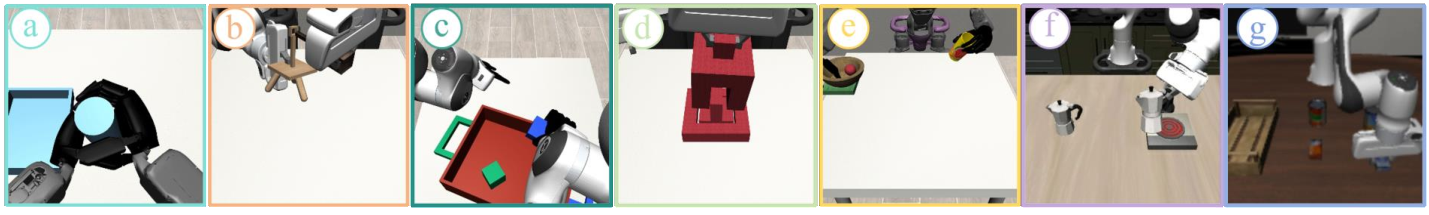
\includegraphics[width=\textwidth]{figure/sim_task.pdf}
\caption{\textbf{Simulated tasks.} The five DexMimicGen simulation tasks, left
to right: the shorter-horizon \textsc{CanSort} control, then four long-horizon dual-arm
tasks \textsc{Threading}, \textsc{LiftTray}, \textsc{PieceAssembly}, and
\textsc{Pouring}.The two LIBERO simulation tasks, left to right: \textsc{Put both moka pots on the stove} as task 8 of LIBERO 10, \textsc{Pick up the cream cheese and put it in the tray} as task 57 of LIBERO 90}
\label{fig:simtask}
\end{figure*}

\begin{figure*}[t]
\centering

\includegraphics[width=\textwidth]{\detokenize{figure/fig_long_horizon_anti_collapse_multiseed_curves copy.pdf}}
\caption{\textbf{Long-horizon simulation results.} Evaluation success rate
versus environment steps on four long-horizon DexMimicGen tasks and the
shorter-horizon \textsc{CanSort} control. Lines are means over three seeds
with $\pm 1$ s.e.m. bands. SHORE-RL is compared with ResFit, DSRL, IBRL,
and full-policy IQL. The thin
gray solid reference in each panel marks that task's mean SHORE-RL success at
zero environment steps, before residual learning.}
\label{fig:main}
\end{figure*}

\paragraph{Tasks and Evaluation.}
We evaluate SHORE-RL on four long-horizon dual-arm dexterous manipulation tasks from
DexMimicGen~\cite{jia2024dexmimicgen,mandlekar2023mimicgen}: \textsc{Threading},
\textsc{LiftTray}, \textsc{PieceAssembly}, and \textsc{Pouring}, plus the
shorter-horizon \textsc{CanSort} control (Fig.~\ref{fig:simtask}). The single-arm
extensions are LIBERO-10 \textsc{Task~8} (\emph{put both moka pots on the stove}) and
LIBERO-90 \textsc{Task~57} (\emph{pick up the cream cheese and put it in the tray})
\cite{liu2023libero} (Fig.~\ref{fig:libero}). We use ACT~\cite{zhao2023learning}
as the base policy for DexMimicGen and $\pi_0$~\cite{black2024pi0} for LIBERO.
DexMimicGen evaluations use $50$ episodes; LIBERO uses $10$ episodes, three seeds,
and $400$k environment steps. Our primary metric, \emph{final-window success}, is
the mean success over the last $20\%$ of evaluations within the stated
comparison budget, reported with seed variation. The learning curves in Fig.~\ref{fig:main} show whether this
performance is sustained or undergoes late-training collapse.

\paragraph{Baselines.}
For the main comparison, we evaluate SHORE-RL against a frozen BC reference
and four RL-finetuning baselines under matched training budgets and evaluation
conditions. \emph{(i)~BC base}: the
frozen base policy with no RL, which determines whether adaptation sustains an
improvement. \emph{(ii)~ResFit}~\cite{resfit2025residual}: a frozen-base
action-residual method that uses equal sampling from offline demonstrations
and online replay.
\emph{(iii)~DSRL}~\cite{wagenmaker2025dsrl}: noise-space RL on the same base,
which tests whether changing the adaptation space prevents late degradation.
\emph{(iv)~IBRL}~\cite{hu2023imitation}: an off-policy method that uses a frozen
BC policy to propose alternative actions for both online action selection and
critic-target bootstrapping. \emph{(v)~IQL}~\cite{kostrikov2022iql}: a
full-policy off-policy RL method that finetunes the entire policy without
retaining a frozen base, included as a non-residual control.

% =====================================================================
% PROVENANCE NOTES for Table 1.
% - IBRL cells use completed 500k-step matched-harness runs: 2 seeds per task,
%   except PieceAssembly with 3 seeds.
% - DSRL and IQL cells are from completed 3-seed runs at 500k steps.
% =====================================================================
\begin{table}[t]
\centering
\setlength{\tabcolsep}{0pt}
\begin{tabular*}{\columnwidth}{@{\extracolsep{\fill}}lcccc}
Method & \textsc{Pouring} & \textsc{PieceAssembly} & \textsc{LiftTray} & \textsc{Threading} \\
\midrule
\textbf{SHORE-RL} & .91 & .66 & .84 & .52 \\
ResFit & .10 & .02 & .03 & .01 \\
DSRL & .26 & .00 & .00 & .00 \\
IBRL & .00 & .10 & .00 & .01 \\
IQL & .00 & .00 & .00 & .40 \\
\bottomrule
\end{tabular*}
\caption{Final-window success for SHORE-RL and four RL-finetuning
baselines on the long-horizon simulation tasks ($50$ episodes per evaluation).
SHORE-RL denotes the main waypoint, demo-BC, and stage-shaping configuration;
all methods use matched training budgets and evaluation conditions.}
\label{tab:main}
\end{table}


% (world-model / real-robot deployment moved to the end of this section, after the sim
% results, so the SHORE-RL sim study reads as the main experiment.)

\paragraph{Sustained Long-Horizon Performance.}
Figure~\ref{fig:main} shows learning curves for four long-horizon tasks and the
shorter-horizon \textsc{CanSort} control, while Table~\ref{tab:main}
summarizes final-window success on the long-horizon tasks. SHORE-RL maintains
high success throughout training on \textsc{Pouring} and \textsc{LiftTray}
and sustains clear improvements on \textsc{PieceAssembly} and
\textsc{Threading}. ResFit, DSRL, IBRL, and full-policy IQL instead finish
below their frozen-base references on the four long-horizon tasks. The late
degradation of full-policy IQL shows that the observed instability is not
limited to residual parameterizations, while the similar degradation of methods
that retain a frozen base policy indicates that such an anchor alone is
insufficient to prevent it. In contrast, ResFit remains
near-optimal on the shorter-horizon \textsc{CanSort} control. Together, the
curves and final-window results support temporal composition as the central
empirical factor and show that SHORE-RL sustains the improvement over its
frozen base across all four long-horizon tasks.

\paragraph{Base Generality: ACT and \textbf{$\pi_0$.}}
Following the frozen-ACT experiments on DexMimicGen, we evaluate SHORE-RL with
a frozen $\pi_0$ VLA on LIBERO-10 \textsc{Task~8} and LIBERO-90
\textsc{Task~57}. Across both tasks, SHORE-RL reaches near-perfect final-window
success under the $400$k-step, three-seed protocol and compares favorably with
DSRL.
Together, the ACT and $\pi_0$ results show that SHORE-RL can be applied to both
tested base-policy classes while retaining competitive performance
(Fig.~\ref{fig:libero}).



\begin{figure}[t]
\centering
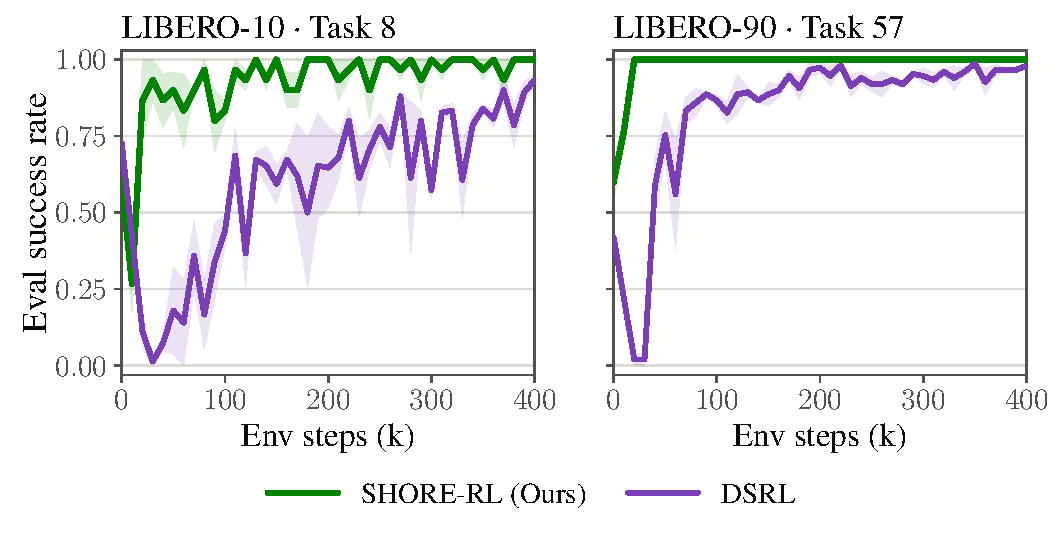
\includegraphics[width=\columnwidth]{figure/fig_libero10_aligned.pdf}
\caption{\textbf{LIBERO $\pi_0$ finetuning.}
Success on LIBERO-10 \textsc{Task~8} (left) and LIBERO-90 \textsc{Task~57}
(right) over $400$k steps. Curves are $3$-seed means with $\pm 1$ s.e.m.
SHORE-RL reaches near-perfect success on both tasks.}
\label{fig:libero}
\end{figure}

\subsection{Ablations}
\label{sec:exp-ablations}

\paragraph{Ablation Setup.}
We evaluate five matched configurations: the full SHORE-RL method and four
ablated variants, each removing one or more components---waypoint conditioning,
demo-BC, and stage shaping---as detailed in Table~\ref{tab:ablarms}.
All configurations use the same codebase, frozen features
$\psi$, offline data, action scale, evaluation protocol, and $400$k-step
training budget. The demo-BC coefficient is $0.1$ except in the configuration that
explicitly removes it. Figure~\ref{fig:ablbars} reports two long-horizon
tasks---\textsc{Pouring} and \textsc{PieceAssembly}---with
three seeds per configuration. For each seed, we average the evaluation success
rates over the final $20\%$ of training; bars report mean$\pm$s.e.\ across these
seed-level averages.

\begin{table}[t]
\centering\small\setlength{\tabcolsep}{4pt}
\resizebox{\columnwidth}{!}{%
\begin{tabular}{@{}lcccl@{}}
\toprule
Configuration & waypoint & BC & staged & removed \\
\midrule
\textbf{SHORE-RL}                       & on  & $0.1$ & on  & ---             \\
w/o stage shaping                       & on  & $0.1$ & off & shaping         \\
w/o waypoint                            & off & $0.1$ & on  & waypoint        \\
w/o waypoint \& stage shaping           & off & $0.1$ & off & both structural \\
w/o demo-BC \& stage shaping            & on  & $0$   & off & BC $+$ staged   \\
\bottomrule
\end{tabular}
}
\caption{Matched component-ablation configurations with fixed action scale, evaluation
protocol, and comparison budget. SHORE-RL uses waypoint conditioning, demo-BC, and the
hand-designed per-stage bonus. The first three variants remove the listed
component or pair of components; the last keeps the waypoint while removing
both demo-BC and stage shaping.}
\label{tab:ablarms}
\end{table}

\paragraph{Component Ablations.}
Figure~\ref{fig:ablbars} summarizes matched component variants under a common
$400$k training budget on two long-horizon tasks. Although both tasks require
extended temporal composition, \textsc{PieceAssembly} represents the more
challenging of the two settings. On \textsc{PieceAssembly}, SHORE-RL reaches
$.65$, whereas every component-removal variant falls to $.14$--$.28$. On
\textsc{Pouring}, SHORE-RL ($.93$) and the variant without waypoint
conditioning ($.92$) are close within seed variation, while the other removals
reach $.73$--$.80$. A plausible explanation is task structure: \textsc{Pouring} is relatively monotone, whereas \textsc{PieceAssembly} requires object- and contact-specific subgoals where waypoint context is more useful. These results reveal non-additive and task-dependent interactions
among waypoint conditioning, behavior anchoring, and stage-based reward
shaping. On \textsc{Pouring}, the waypoint-only variant reaches $.78$;
together with the low late-training ResFit performance in
Figure~\ref{fig:main}, this suggests that waypoint conditioning is useful even
without the other two components. Meanwhile, the combination of demo-BC and
stage shaping reaches $.92$ without waypoint conditioning, close within seed
variation to the full method at $.93$. This small conditional gap does not
imply that waypoint conditioning is ineffective; rather, it indicates that the
other two components can compensate for part of its contribution on this task.
On \textsc{PieceAssembly}, neither waypoint conditioning alone ($.23$) nor
demo-BC combined with stage shaping ($.28$) approaches the full method
($.65$), indicating substantially stronger complementarity among the
components. Overall, the components do not provide independent additive gains:
their effects depend on both the other active components and the task, while
the complete configuration provides the strongest and most robust performance
across the two long-horizon tasks.

\begin{figure}[tbp]
\centering
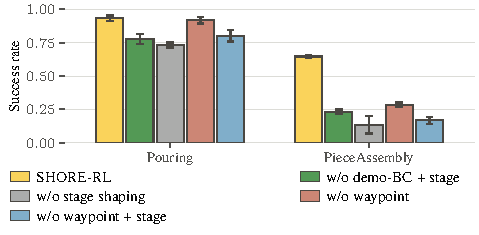
\includegraphics[width=0.90\columnwidth]{figure/fig_ablation_bars_400k.pdf}
\caption{\textbf{Ablation~A: matched component ablation.}
Success on two long-horizon dual-arm tasks with a common $400$k training
budget. Each per-seed score averages the evaluation success rates over the
final $20\%$ of training. Bars show means across three seeds, and error bars
show $\pm 1$ s.e.m.}
\label{fig:ablbars}
\end{figure}

\paragraph{Reward Form: Stage Bonus vs.\ Self-Derived Potential.}
\begin{figure}[!b]
\centering
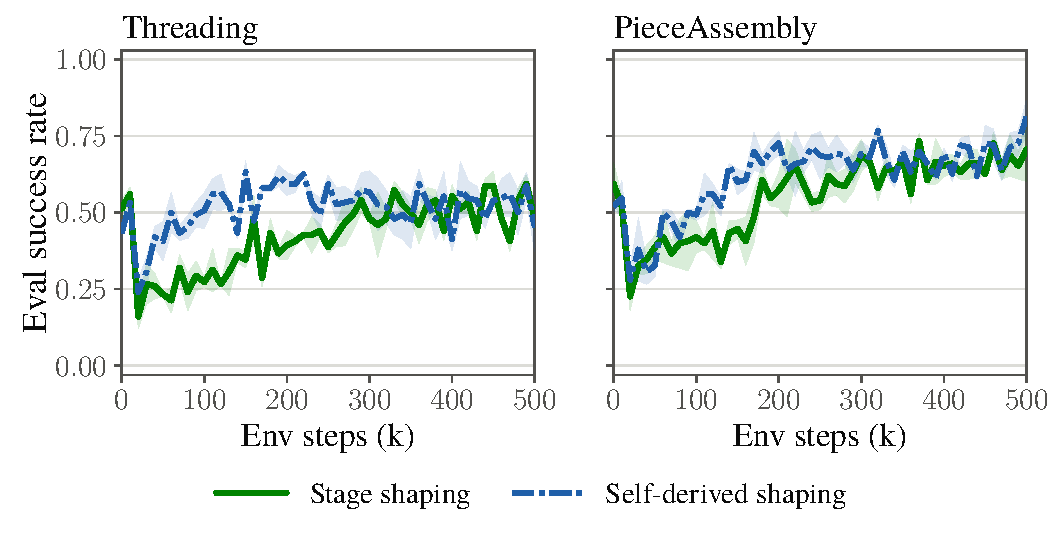
\includegraphics[width=\columnwidth]{figure/fig_staged_vs_pothiql_threading_piece_v2.pdf}
\caption{\textbf{Ablation~B: stage bonus vs.\ self-derived potential.}
Evaluation success versus environment steps on two stage-structured
long-horizon tasks. Both variants use waypoint conditioning, demo-BC, and online
joint finetuning; they differ only in the critic reward. \emph{Stage shaping}
uses the hand-designed per-stage bonus, whereas \emph{Self-derived shaping}
uses potential differences from $V_{\mathrm p}$. Lines are three-seed means
with $\pm 1$ s.e.m. bands.}
\label{fig:stagevspot}
\end{figure}


\begin{figure*}[!t]
\centering
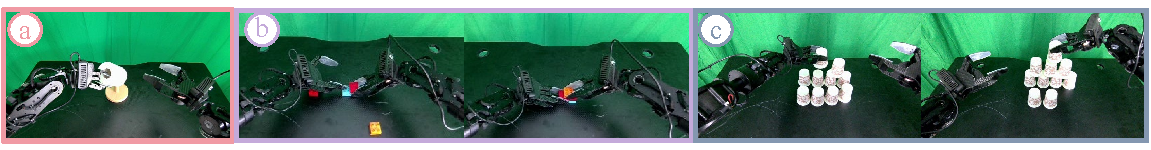
\includegraphics[width=\textwidth]{figure/real_task.pdf}
\caption{\textbf{Real-robot tasks.} Three bimanual tabletop tasks:
(a)~\textsc{Paper-Roll Placement}: picking up a paper roll and placing it
onto a holder; (b)~\textsc{Block Assembly}: assembling toy blocks; and
(c)~\textsc{Cup Stacking}: stacking paper cups into four levels.}
\label{fig:realtask}
\end{figure*}

\begin{figure*}[!t]
\centering
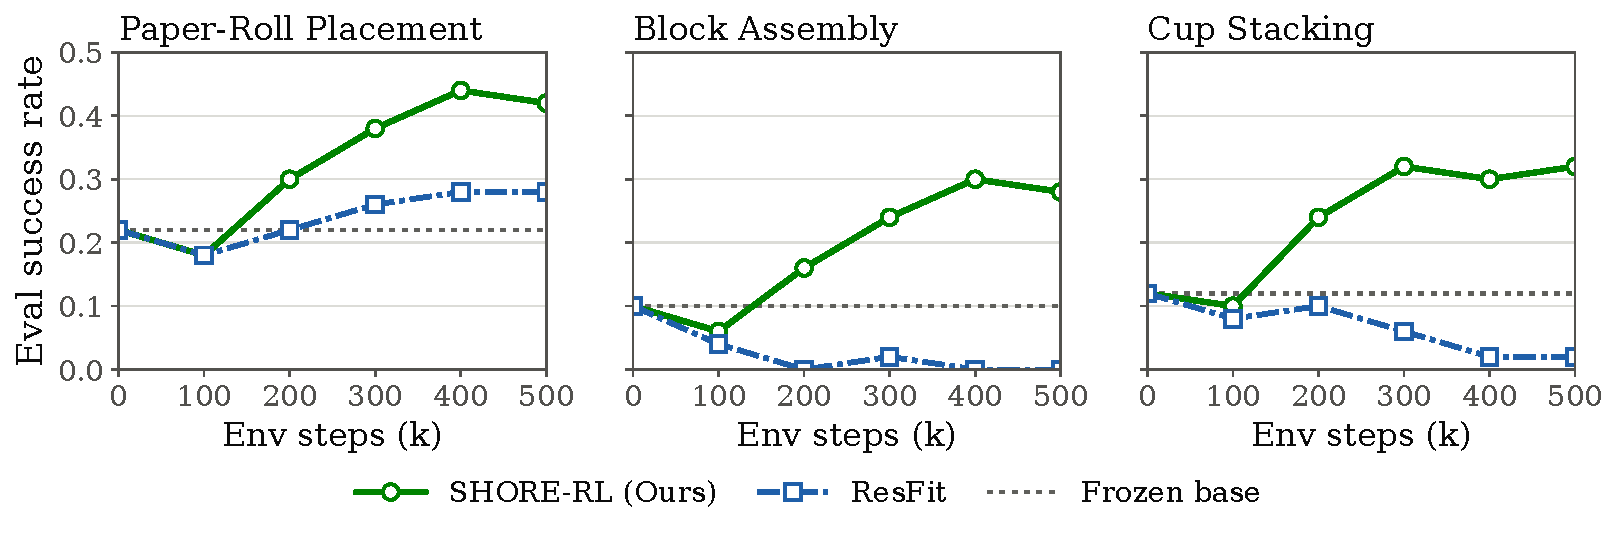
\includegraphics[width=0.85\textwidth]{figure/fig_real_robot_curves.pdf}
\caption{\textbf{Real-robot learning curves.} Success rates over six checkpoints; green is SHORE-RL, blue is ResFit, and gray is the frozen base.}
\label{fig:realrobot-curves}
\end{figure*}

The main long-horizon study uses a hand-designed per-stage signal, whose
limitation is the need for a task-specific phase detector and a predefined
decomposition. We test whether the detector can be removed while holding the
rest of SHORE-RL fixed. The self-derived alternative uses the
separate single-state value $V_{\mathrm p}$ trained from the same frozen
features and demonstrations, and changes only the critic reward source.
Figure~\ref{fig:stagevspot} gives the controlled comparison on the two
stage-structured tasks. Final-window success with $V_{\mathrm p}$ is
indistinguishable from stage shaping on \textsc{Threading} ($.52$ vs.\ $.52$)
and is numerically higher on \textsc{PieceAssembly} ($.70$ vs.\ $.66$).
Both panels use three seeds. These results support self-derived potential
shaping as a replacement for the hand-designed stage bonus, removing the need
for a hand-written stage detector in the tested settings.







\subsection{Real-Robot Experiments}
\label{sec:exp-real}
\paragraph{Platform.}
We use a full-body robot with two $7$-DoF arms and parallel grippers, yielding a
$16$-D joint-and-gripper action space. Observations are three $848{\times}480$
RGB streams at $30$\,Hz. Each task uses a frozen served
$\pi_{0.5}$-style VLA~\cite{sima2026kai0} that outputs $50$-step action chunks.

\paragraph{Tasks and Pipeline.}
The three bimanual tasks are \textsc{Paper-Roll Placement}, \textsc{Block
Assembly}, and \textsc{Cup Stacking} (Fig.~\ref{fig:realtask}). They
respectively require picking up and placing a paper roll onto a holder,
assembling toy blocks, and stacking paper cups into a four-level structure.
For each task,
we first collect about $1{,}000$ successful teleoperated episodes. These
demonstrations are used to finetune a task-specific $\pi_{0.5}$ base, which is
then frozen. We next deploy each frozen base to collect additional rollouts,
including observed failures. Finally, we pool the demonstrations and
base-policy rollouts from all three tasks to finetune a single dynamics model
$D$ shared across tasks. After
finetuning, $D$ is frozen and used only to generate imagined rollouts for
residual training. At each rollout step, the frozen base and
waypoint-conditioned residual jointly produce an action chunk, $D$ predicts
the resulting future observations, and the self-derived potential provides the
critic reward for residual updates. At deployment, the frozen base is
augmented by the trained SHORE-RL residual, while $D$ is not used.

\paragraph{Evaluation.}
We compare the frozen base, ResFit, and SHORE-RL using the same base,
observation interface, and fixed physical initial-state set.
Figure~\ref{fig:realrobot-curves} tracks evaluation success at six checkpoints
from step~$0$ to $500$k. After a small initial dip, SHORE-RL improves on all
three tasks and finishes above both its frozen base and ResFit. At $500$k,
SHORE-RL reaches $.42$ on \textsc{Paper-Roll Placement}, $.28$ on
\textsc{Block Assembly}, and $.32$ on \textsc{Cup Stacking}, compared with
frozen-base success rates of $.22$, $.10$, and $.12$. ResFit improves over the
frozen base only on \textsc{Paper-Roll Placement}, reaching $.28$, but declines
to $.00$ and $.02$ on \textsc{Block Assembly} and \textsc{Cup Stacking}.
Table~\ref{tab:realrobot} summarizes the step-$0$ frozen-base results and the
$500$k adapted results. Each reported value is computed from $50$ physical
robot trials.

\begin{table}[!t]
\centering\small\setlength{\tabcolsep}{4pt}
\begin{tabular}{@{}lccc@{}}
\toprule
Task & Frozen Base & ResFit & \textbf{SHORE-RL} \\
\midrule
\textsc{Paper-Roll Placement} & .22 & .28 & \textbf{.42} \\
\textsc{Block Assembly}       & .10 & .00 & \textbf{.28} \\
\textsc{Cup Stacking}         & .12 & .02 & \textbf{.32} \\
\bottomrule
\end{tabular}
\caption{Real-robot success rates. Frozen base is step $0$; ResFit and SHORE-RL are at $500$k, with $50$ physical trials per cell.}
\label{tab:realrobot}
\end{table}

% =====================================================================
\section{Conclusion}
% =====================================================================
SHORE-RL shortens residual BC finetuning with base-feature waypoints and a
separate dense critic-reward path. Across four long-horizon DexMimicGen tasks,
it sustains improvements while the tested RL-finetuning baselines collapse below
their frozen bases. A self-derived potential also matches or exceeds the stage
bonus on two stage-structured tasks, reducing reliance on hand-written stage
detectors.

\clearpage
% NOTE: aaai2027.sty auto-sets \bibliographystyle when natbib is loaded; do NOT add it here.
\bibliography{references}

\end{document}
